\documentclass[
12pt,
a4paper,
pdftex,
czech,
titlepage
]{report}

\usepackage[czech]{babel}
\usepackage[utf8]{inputenc}
\usepackage{lmodern}
\usepackage{textcomp}
\usepackage[T1]{fontenc}
\usepackage{amsfonts}
\usepackage{titlesec}
\usepackage{graphicx}
\usepackage{listings}
\usepackage{color}
\usepackage{hyperref}
\usepackage{listings}

\definecolor{dkgreen}{rgb}{0,0.6,0}
\definecolor{gray}{rgb}{0.5,0.5,0.5}
\definecolor{mauve}{rgb}{0.58,0,0.82}

\lstset{frame=tb,
  language=C,
  aboveskip=3mm,
  belowskip=3mm,
  showstringspaces=false,
  columns=flexible,
  basicstyle={\small\ttfamily},
  numbers=none,
  numberstyle=\tiny\color{gray},
  keywordstyle=\color{blue},
  commentstyle=\color{dkgreen},
  stringstyle=\color{mauve},
  breaklines=true,
  breakatwhitespace=true,
  tabsize=3
}


\titleformat{\chapter}
  {\normalfont\LARGE\bfseries}{\thechapter}{1em}{}
\titlespacing*{\chapter}{0pt}{0ex plus 1ex minus .2ex}{2.0ex plus .2ex}

\begin{document}

\begin{titlepage}
	\vspace*{-2cm}
	{\centering
\includegraphics[scale=1.0]{logo.pdf}\par}
	\centering
	\vspace*{2cm}
	{\Large Semestrální práce z KIV/FJP\par}
	\vspace{1.5cm}
	{\Huge\bfseries Tvorba dat pro program IMiGEr\par}
	\vspace{2cm}

	{\Large Vít Mazín, Martin Matas\par}
	{\Large A18N0096P, A18N0095P\par}
	{\Large mazinv@students.zcu.cz, martinm@students.zcu.cz\par}

	\vfill

	{\Large 20.\,11.\,2018}
\end{titlepage}

\tableofcontents
\thispagestyle{empty}
\clearpage

\chapter{Zadání}
\setcounter{page}{1}
\paragraph{\parindent=4em}{
Tématem semestrální práce bude převedení SLR gramatik do formátu JSON, který je zobrazen ve vizualizačním nástroji IMiGEr vytvořeným na Katedře informační a výpočetní techniky.
}

\chapter{Analýza}
\section{Způsob přečtení SLR gramatik}
\paragraph{\parindent=4em}{
Během analýzy výstupu programu Bison bylo zjištěno, že Bison umožňuje danou gramatiku převést do formátu \textbf{DOT} (graph description language). Tento formát je následně možné vizualizovat nástrojem Graphviz. Tímto lze výstupní automat zobrazit jako graf. Tento formát však není podporován nástrojem IMiGEr, proto bylo nutné najít cestu jak formát převést do požadovaného tvaru. Původní myšlenkou byla tvorba vlastního parseru. Při bližší analýze formátu jsme objevili existující knihovnu \textbf{digraph-parser} pro jazyk Java, která umožňuje uložený graf přečíst a vytvořit objekty z jeho vrcholů a hran.
}
\subsection{Formát DOT}
\paragraph{\parindent=4em}{
V následující ukázce je vidět struktura formátu DOT.
}
\begin{lstlisting}
graph graphname {
     // This attribute applies to the graph itself
     size="1,1";
     // The label attribute can be used to change the label of a node
     a [label="Foo"];
     // Here, the node shape is changed.
     b [shape=box];
     // These edges both have different line properties
     a -- b -- c [color=blue];
     b -- d [style=dotted];
     // [style=invis] hides a node.
   }
\end{lstlisting}   

\section{Způsob uložení gramatiky do formátu JSON}
\paragraph{\parindent=4em}{
Požadovaný výstupní formát byl fomrát JSON. Pro převedení objektů jazyka Java do formátu JSON byla zvolena knihovna \textbf{Jackson}. Přesná podoba jak má být graf reprezentován ve formátu JSON je přiložena v repozitáři programu IMiGEr na portále \textbf{\href{https://github.com/ReliSA/IMiGEr/blob/master/documents/IMiGEr/IMiGEr\_raw\_input\_format.pdf}{GitHub}}.
}

\chapter{Programová dokumentace}
\section{Úvod}
\paragraph{\parindent=4em}{
Pro implementaci nástroje jsme zvolili programovací jazyk Java. Byly použity knihovny \textbf{digraph-parser} a \textbf{Jackson}. Aplikace sestává z 5 následujících balíků:

\begin{description}
 \item[cz.zcu.kiv.fjp] \hfill \\ Obsahuje hlavní třídu aplikace, která se stará o její správné spuštění a volá programové API.
 \item[cz.zcu.kiv.fjp.core] \hfill \\ API aplikace, které volá metody z balíků parser a serializer.
 \item[cz.zcu.kiv.fjp.core.entities] \hfill \\ Jednotlivé entity, které vnitřně reprezentují načtený graf, např. vrchol, hrana, atributy.
 \item[cz.zcu.kiv.fjp.core.parser] \hfill \\ Balík obsahuje parser umǒžňující zpracovat jak SLR gramatiku, tak i obecný a vnitřně je reprzentovat s využitím entit.
 \item[cz.zcu.kiv.fjp.core.serializer] \hfill Slouží k převodu vnitřní reprezentace grafu do formátu JSON, který byl specifikován výše.
\end{description}
}

\section{Běh programu}
\paragraph{\parindent=4em}{
Program nejprve v hlavní třídě \texttt{Main} zpracuje argumenty programu a poté podle nich volá API, jež ja naprogramováno v třídě \texttt{core.Dot2JSON}.
}

\paragraph{\parindent=4em}{
Následně se zpracuje vstupní .dot soubor příslušným parserem z balíku \texttt{core.parser}, který dědí abstraktní třídu \texttt{DotParser}. Pro obecné grafy je to \texttt{GeneralParser} a pro grafy vytvořené ze SLR gramatik je to \texttt{SLRParser}. Výstupem jsou kolekce vrcholů a hran grafu.
}

\paragraph{\parindent=4em}{
Dále jsou kolekce vrcholů a grafů serializovány příslušnoým serializérem z balíku \texttt{core.serializer}, který implementuje rozhraní \texttt{IDotSerializer}. Konkrétně se jedná o třídu \texttt{DotSerializer}. Tato třída uloží data do výstupního souboru formátu JSON.
}

\paragraph{\parindent=4em}{
Na následujícím UML diagramu \ref{fig:uml} je znázorněna závislost tříd programu. Diagram je ochuzen o některé třídy z balíku \texttt{core.entities}, které specifikují vlastnosti vrcholů a hran. Tyto třídy byly vytvořeny pro potřeby serializace.

\begin{figure}[!h]
  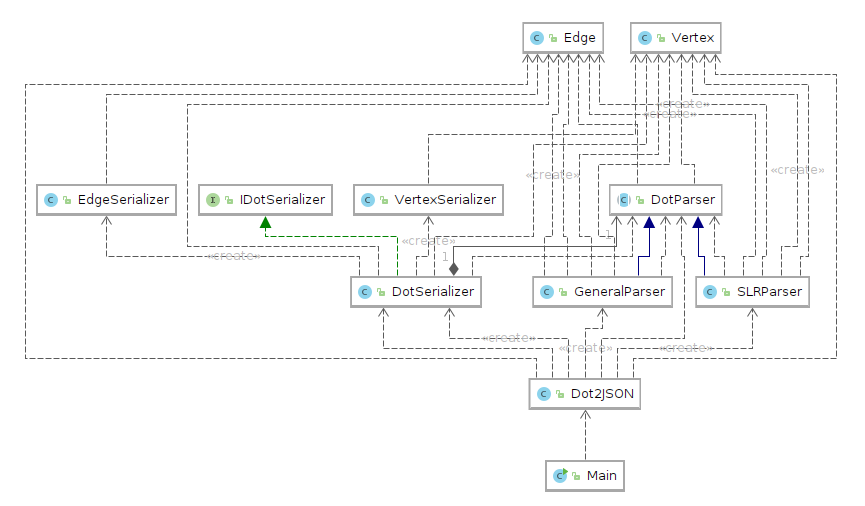
\includegraphics[width=\linewidth]{uml_diagram}
  \caption{UML diagram programu (zjednodušeno)}
  \label{fig:uml}
\end{figure}
}

\chapter{Uživatelská dokumentace}
\section{Spuštění programu}
\paragraph{\parindent=4em}{
Program přeložený jako .jar archiv lze spustit ve dvou režimech. V prvním je zadán pouze název a cesta vstupního .dot souboru a název s cestou výstupního .json souboru. V tomto režimu program převádí obecné grafy do požadovaného výstupního formátu. Program v prvním režimu lze spustit například takto:\\
\texttt{java -jar SLR-visualization-for-IMiGEr.jar input.dot output.json}\\


V druhém režimu program převádí do požadovaného výstupu grafy, které vytvoří program Bison. Ten ukládá do formátu .dot automat dané SLR gramatiky. Jako argumenty je nutné zadat přepínač \texttt{--slr} a poté zadat vstupní .dot soubor a výstupní .json soubor. Program v druhém režimu lze spustit například takto:\\
\texttt{java -jar SLR-visualization-for-IMiGEr.jar input.dot output.json}\\


Pokud nejsou zadány požadované argumenty, program napoví, že ho lze spustit s přepínačem \texttt{-h}, který zobrazí nápovědu jak program korektně spustit.
}

\chapter{Závěr}
\paragraph{\parindent=4em}{
Domníváme se, že naše zadání bylo splněno. Program korektně převádí grafy, jež jsou výstupem programu Bison a navíc také dokáže převést libovolný graf, který je ve formátu DOT do požadovaného výstupního JSON formátu. Program lze použít samostatně nebo jako knihovnu, jež ze vstupního souboru poskytne informace o vrcholech a hranách grafu.
}

\end{document}